%File: main.tex
%====================================================================
% AAAI-style FINAL REPORT for the HC-RAG project (v3, Amazon-focused).
% Authors: Ben Volovelsky, Noam Delbari.
% ALL numbers are REAL (Amazon report + HC_vs_Baselines + HC_RESULTS_REPORT + FiQA).
%====================================================================

\documentclass[letterpaper]{article}
\usepackage{aaai}
\usepackage{times}
\usepackage{helvet}
\usepackage{courier}
\usepackage{graphicx}
\usepackage{booktabs}
\usepackage{array}
\usepackage{float}
\usepackage{amsmath}
\usepackage{amssymb}
\usepackage{enumitem}
\usepackage{url}
\frenchspacing
\setlength{\pdfpagewidth}{8.5in}
\setlength{\pdfpageheight}{11in}

\pdfinfo{
/Title (Higher Criticism for Adaptive Retrieval: A Controlled Study of Null Calibration)
/Author (Lihu Zur and Noam Delbari)
/Keywords (Retrieval-Augmented Generation, Higher Criticism, Adaptive Retrieval, Null Calibration, Information Retrieval)
}

\setcounter{secnumdepth}{2}

%====================================================================
% === Numbered references (override aaai.sty author-year style) ===
%====================================================================
\makeatletter
\def\@biblabel#1{[#1]}
\def\@cite@ofmt{\hbox}
\def\@cite#1#2{[{#1\if@tempswa , #2\fi}]}
\def\@citex[#1]#2{%
  \let\@citea\@empty
  \@cite{\@for\@citeb:=#2\do
    {\@citea\def\@citea{,\penalty\@m\ }%
     \edef\@citeb{\expandafter\@firstofone\@citeb\@empty}%
     \if@filesw\immediate\write\@auxout{\string\citation{\@citeb}}\fi
     \@ifundefined{b@\@citeb}{\mbox{\reset@font\bfseries ?}%
       \G@refundefinedtrue
       \@latex@warning{Citation `\@citeb' on page \thepage \space undefined}}%
       {\@cite@ofmt{\csname b@\@citeb\endcsname}}}}{#1}}
\DeclareRobustCommand\cite{\@ifnextchar[{\@tempswatrue\@citex}{\@tempswafalse\@citex[]}}
\def\thebibliography#1{\section*{References}%
  \@mkboth{REFERENCES}{REFERENCES}%
  \list{\@biblabel{\@arabic\c@enumiv}}%
    {\settowidth\labelwidth{\@biblabel{#1}}%
     \leftmargin\labelwidth \advance\leftmargin\labelsep
     \usecounter{enumiv}\let\p@enumiv\@empty
     \renewcommand\theenumiv{\@arabic\c@enumiv}}%
  \sloppy\clubpenalty4000\widowpenalty4000\sfcode`\.\@m}
\let\endthebibliography=\endlist
\makeatother

%====================================================================
% === Editable Numbers (REAL) ===
%====================================================================
% city-retrieval benchmark
\newcommand{\CatHCR}{0.852}\newcommand{\CatHCP}{0.938}\newcommand{\CatHCF}{0.893}
\newcommand{\CatHCK}{9.7}\newcommand{\CatCorrK}{0.835}\newcommand{\CatTenF}{0.783}
% category-and-price corpus failure decomposition
\newcommand{\AmFailN}{55}\newcommand{\AmTotN}{135}
\newcommand{\AmIrrN}{24}\newcommand{\AmFixN}{31}\newcommand{\AmPosN}{77}
\newcommand{\AmSigQ}{1.74}\newcommand{\AmSigNull}{2.06}\newcommand{\AmStdCorr}{0.83}
% algorithm comparison (pool N=1000)
\newcommand{\AlgHCF}{0.209}\newcommand{\AlgHCK}{34.0}\newcommand{\AlgBJF}{0.202}
\newcommand{\AlgTwentyF}{0.185}\newcommand{\AlgFiftyF}{0.187}
\newcommand{\AlgAdaKF}{0.138}\newcommand{\AlgCARF}{0.110}
\newcommand{\AlgBHF}{0.074}\newcommand{\AlgBonfF}{0.022}
% electronics corpus
\newcommand{\AmElHCF}{0.192}\newcommand{\AmElTwentyF}{0.185}\newcommand{\AmElFiftyF}{0.166}
\newcommand{\AmElTokF}{15.0}\newcommand{\AmElTitleF}{19.6}\newcommand{\AmElFuzzyF}{17.0}
% Phase 1: BM25 / Adaptive-RAG
\newcommand{\CEqaFHC}{0.620}\newcommand{\CEqaFoner}{0.609}\newcommand{\CEqaFircot}{0.540}
\newcommand{\MusFHC}{0.301}\newcommand{\MusFoner}{0.301}\newcommand{\MusFircot}{0.315}
% Phase 1: dense Adaptive-K
\newcommand{\HotFHC}{0.332}\newcommand{\HotFAdaK}{0.306}
\newcommand{\HotEMHC}{0.150}\newcommand{\HotEMAdaK}{0.122}
\newcommand{\HotPrecHC}{0.221}\newcommand{\HotPrecAdaK}{0.020}
\newcommand{\HolJHC}{0.321}\newcommand{\HolJAdaK}{0.326}
\newcommand{\HolPrecHC}{1.000}\newcommand{\HolPrecAdaK}{0.531}
% Phase 1: FiQA
\newcommand{\FqBaseNDCG}{0.362}\newcommand{\FqHCNDCG}{0.418}
\newcommand{\FqBasePre}{0.171}\newcommand{\FqHCPre}{0.319}
\newcommand{\FqJudgeWin}{44.8}\newcommand{\FqJudgeLose}{34.7}

%====================================================================
% === Title and Author ===
%====================================================================
\title{Higher Criticism for Adaptive Retrieval:\\From Pipeline Integration to a Controlled Study of Null Calibration}
\author{Lihu Zur \and Noam Delbari\\
Final Project Report\\
\texttt{lihu.zur@post.runi.ac.il} \quad \texttt{noam.delbari@post.runi.ac.il}\\
}

\begin{document}
\maketitle

%====================================================================
% === Abstract ===
%====================================================================
\begin{abstract}
Retrieval-Augmented Generation (RAG) usually retrieves a fixed number of
passages per query, spending context on easy questions while
under-serving hard ones. Higher Criticism (HC) is a statistical test for
rare, weak signals that turns this fixed choice into a query-adaptive
cutoff: similarity scores become $p$-values under a null distribution,
and HC keeps the documents whose scores are too high to come from the
irrelevant background. Across three existing RAG pipelines and a
controlled study on our own, HC is the strongest adaptive cutoff we
tested. On multi-hop QA it improves answer Exact Match by 23\% over the
gap-based adaptive-retrieval baseline and raises context precision more
than tenfold, while reading an order of magnitude less context. On a
controlled product-retrieval benchmark a single global null instead makes
HC collapse on 55 of 135 queries; we trace this to a per-query scale
mismatch and correct it with a label-free recalibration that needs no
labels and keeps one global null, recovering 97\% of the fixable queries
and giving HC the best retrieval F1 of eight methods, 12\% above the best
fixed cut. The advantage carries to end-to-end RAG, where HC improves
answer token-F1 by 15\% over a fixed Top-20, and holds from 726 documents
to 100{,}000.
\end{abstract}

%====================================================================
% === Background and Motivation ===
%====================================================================
\section{Background and Motivation}
Retrieval-Augmented Generation (RAG) \cite{lewis2020rag} grounds a large
language model (LLM) in passages pulled from an external corpus by an
approximate-nearest-neighbour search. The dominant interface is
\emph{Top-$k$}: fix an integer $k$ and pass the $k$ highest-scoring
passages to the generator. This is convenient but blunt. A single $k$
cannot serve a fact-lookup query that needs one passage, a multi-hop
question that needs a handful, and a database-style aggregation that
needs dozens. Because the number of genuinely relevant passages varies
enormously across queries, one fixed $k$ is wrong for most queries at
once: too small a value discards evidence, while too large a value floods
the prompt with distractors, inflating cost and degrading answers. What
the retriever needs is not a better fixed $k$ but a per-query rule that
decides, from the scores themselves, where the relevant passages stop.

\subsection{Retrieval as Sparse Signal Detection}
\label{sec:sparse}
A query-aware retriever maps every document in the corpus to a similarity
score against the query. The overwhelming majority of those scores come
from \emph{irrelevant} passages and together form a background null
distribution; only a small, query-dependent number of relevant passages
(the \emph{signals}) are pushed above it. Choosing $k$ is then a
\emph{detection} problem rather than a ranking one: how many of the top
scores are too high to be explained by the irrelevant background? This is
the rare/weak-signal mixture problem that Higher Criticism was designed
for, with documents in place of features and an empirical similarity null
in place of an analytic Gaussian null.

\begin{figure}[t]
\centering
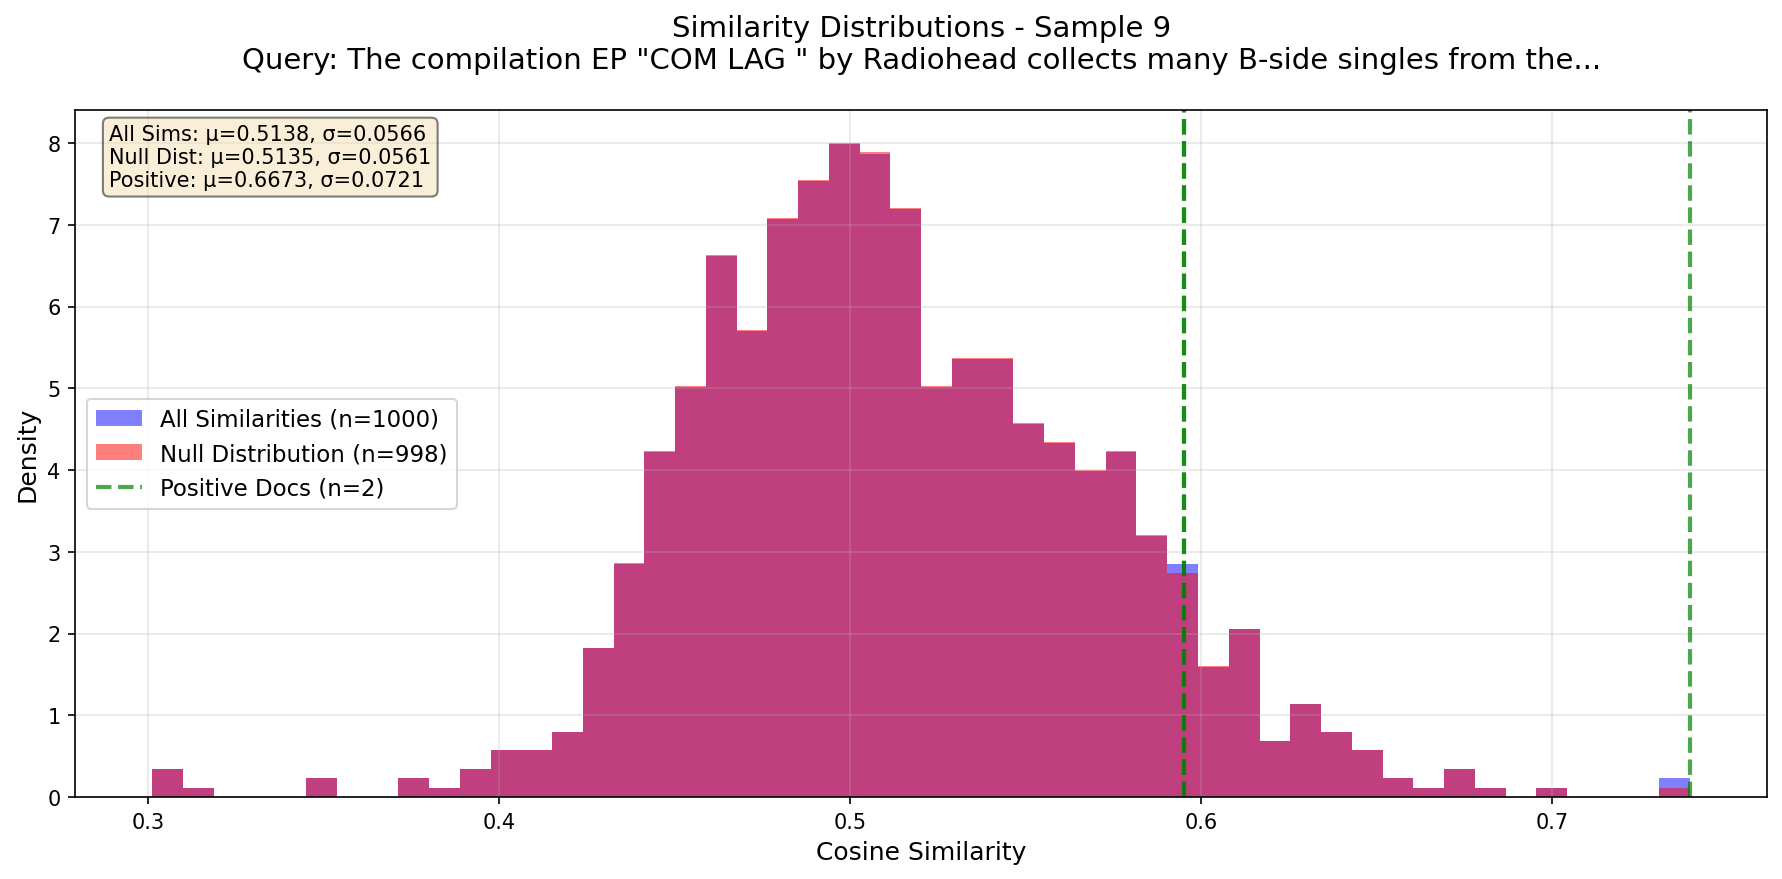
\includegraphics[width=\linewidth]{figures/plot_a_similarities_sample_9.png}
\caption{Retrieval as sparse signal detection (one HotpotQA query). The
few relevant documents (green) sit in the right tail of a large null of
irrelevant similarity scores; HC locates where that tail stops being
explainable by the null.}
\label{fig:signaldetection}
\end{figure}

\subsection{Higher Criticism as a Cutoff Rule}
\emph{Higher Criticism} (HC) \cite{donohojin2004hc} is a goodness-of-fit
statistic for detecting a small number of weak signals in a sea of nulls.
Given a pool of $N$ candidate documents with similarity scores
$s_1 \ge \dots \ge s_N$, we convert each $s_i$ to a $p$-value $p_i$ under
a calibrated null. The $p$-value of a (query, document) pair is the
probability of observing a similarity at least as high as $s_i$ between
the query and a randomly drawn \emph{irrelevant} passage, so a small
$p_i$ means the document is too similar to be a noise hit. Sorting
$p_{(1)} \le \dots \le p_{(N)}$, the HC statistic at rank $i$ is
\[
\mathrm{HC}_i \;=\; \sqrt{N}\;
\frac{i/N - p_{(i)}}{\sqrt{p_{(i)}(1-p_{(i)})}},
\]
which compares the empirical order-statistic quantile $p_{(i)}$ with its
expectation $i/N$ under the null, where the $p$-values would be i.i.d.\
uniform. A large positive $\mathrm{HC}_i$ means the top-$i$ scores are
systematically more extreme than the null predicts, and the adaptive
cutoff is $k^\star = \arg\max_i \mathrm{HC}_i$. We bound the search to the
top $\gamma$ fraction of the pool only as a guardrail: at the very
smallest ranks the denominator $\sqrt{p_{(i)}(1-p_{(i)})}$ is tiny, so a
single outlier can create a spurious maximum. The $\gamma$ window simply
excludes that unstable tail and does not otherwise shape the selection.

\subsection{The Null Distribution}
Every quantity above is anchored to one object: the null distribution of
similarity scores for irrelevant query--document pairs. It is the
reference against which an observed score is judged extreme. We build it
once, offline, by sampling many random pairings of a query with documents
that are not relevant to it and standardizing the resulting similarities
to $z$-scores, so that a single calibrated distribution summarizes what a
typical irrelevant match looks like. At inference, an observed score
$s_i$ is mapped to its $p$-value as the null's tail mass above $s_i$, and
those $p$-values feed the HC statistic. Because the $p$-values, the $i/N$
comparison, the location of the maximum, and hence $k^\star$ all derive
from this one mapping, the null is the single object that determines the
entire cutoff. A retriever meant for deployment calibrates it once and
must apply it to queries it has never seen, so the production-realistic
requirement is a single \emph{global} null shared by all queries.
Per-query nulls are a controlled-lab convenience, not a deployable
design, and the global null is the realistic constraint under which HC
must operate.

\subsection{Research Question}
Our objective is not merely to benchmark HC but to understand
\emph{when} an HC-driven cutoff helps and to characterize and repair the
cases where it does not, asking how the global null fails when its
conditions break and whether those failures can be diagnosed from
observable pool statistics and corrected without per-query labels. The
report also responds to the feedback from our final project presentation,
which asked us to frame retrieval as sparse signal detection, explain the
(query, document) $p$-value, separate methodology from results, and, as
its central scientific point, verify that the $p$-values are uniform
under the null. That concern arose because our early results showed HC
behaving more conservatively (higher precision, lower recall) than its
theory predicts; Section~\ref{sec:amazon} and \ref{app:null}
address it directly.

%====================================================================
% === Methodology ===
%====================================================================
\section{Methodology}

\subsection{HC Retrieval Algorithm}
The HC cutoff has two parts: an offline calibration of the null and an
online selection rule. Offline, we sample random (query, non-relevant
passage) pairs, standardise their similarity scores to $z$-scores, and
fit the empirical CDF of that pooled distribution. This single calibrated
null, shared by every query at inference, is the deployable object: a
production retriever calibrates once and must then generalise to unseen
queries, so we hold the null fixed rather than re-estimating it per
query. Online, for a query we retrieve a candidate pool, map each score
to a $z$-score, and pass it through the null's empirical CDF to obtain a
$p$-value. Sorting the $p$-values, we take the cutoff
$k^\star = \arg\max_i \mathrm{HC}_i$ (with the $\gamma$ guardrail of
Section~\ref{sec:sparse}) and return the top-$k^\star$ passages. Because
the null governs every $p$-value, its fidelity to the current query's
irrelevant scores is what decides whether the cutoff is well placed;
Section~\ref{sec:amazon} traces essentially all of HC's failures to this
object and repairs them without abandoning the global null. The cutoff is
a drop-in stage, so every pipeline we evaluate differs only in this box;
the full offline/online pipeline is diagrammed in
\ref{app:pipeline}.

\subsection{Methods and Pipelines}
We treat HC as one selection rule among a family that turns a candidate
pool into a retrieved set, spanning three design philosophies. The
\emph{rank-based} rule is fixed Top-$k$, which ignores the score
distribution. The \emph{geometric} rules cut on the shape of the sorted
scores: gap-based Adaptive-K \cite{adaptivek2025} cuts at the largest
score gap and clustering-based CAR \cite{xu2025car} at a cluster
boundary, while Adaptive-RAG \cite{jeong2024adaptiverag} routes each
query by predicted complexity. The \emph{statistical} rules operate on
the same $p$-values as HC: Bonferroni \cite{bonferroni1961dunn} and
Benjamini--Hochberg \cite{benjamini1995fdr} threshold individual
$p$-values to control the family-wise error and false discovery rates,
while Berk--Jones \cite{berkjones1979} and HC \cite{donohojin2004hc}
aggregate the whole ordered set into a goodness-of-fit deviation from the
uniform null. Holding the pool and the $p$-value machinery fixed isolates
the selection rule as the axis of comparison; the full method-by-method
table is in \ref{app:methods}.

\subsection{Datasets and Setup}
The study runs in two phases that serve different purposes
(Table~\ref{tab:datasets}). Phase~1 tests HC inside three existing
pipelines it did not control and across standard benchmarks; these fix
the retriever and answerer, so they measure the end-to-end value of an
adaptive cutoff but do not let us instrument the null. Phase~2 isolates
mechanism on our own pipeline, where every document's relevance and every
query's true number of relevant passages are fixed by construction, so
each outcome can be attributed to a specific cause. Phase~2 is organised
around one design principle: each benchmark is built so that a dense
embedder cannot separate relevant from non-relevant documents by
semantics alone, which keeps the task from being solved by plain
nearest-neighbour ranking and genuinely exercises HC's statistical
selection. It starts with a controlled \emph{city-retrieval benchmark} of
``largest cities in [country]'' queries, where embeddings do separate
relevant from irrelevant cleanly and a correctly calibrated cutoff should
work. It then moves to product corpora whose queries pair a category with
a price constraint (for example, ``electronics under \$150''): price is
an attribute the text embedding does not encode, so items in the right
category at the wrong price sit among the relevant ones and cannot be
ranked apart by similarity. We report retrieval Recall/Precision/F1 and
the mean adaptive $k$, and, where a generator is in the loop, answer EM
and token-F1.

\begin{table}[t]
\centering\small
\setlength{\extrarowheight}{1pt}
\begin{tabular}{|p{0.32\linewidth}|c|c|p{0.24\linewidth}|}
\hline
\textbf{Dataset} & \textbf{Docs} & \textbf{Queries} & \textbf{Relevant / query} \\
\hline
\multicolumn{4}{|l|}{\emph{Phase 1: HC inside three existing pipelines}}\\
\hline
CrossEntityQA (ours) & 13K & 105 & variable, 2--20 \\
\hline
MuSiQue & 139K & 500 & 1--4 \\
\hline
HotpotQA & 2K & 987 & $\sim$2 \\
\hline
HoloBench & 260 & 90 & $\sim$152 \\
\hline
BEIR FiQA & 58K & 648 & scattered \\
\hline
\multicolumn{4}{|l|}{\emph{Phase 2: controlled study on our own pipeline}}\\
\hline
City benchmark & 726 & 44 & variable, 4--24 \\
\hline
Category+price products & 80K & 135 & $\sim$4.8\% \\
\hline
Electronics products & 100K & 44 & $\sim$1.2\% \\
\hline
\end{tabular}
\caption{The evaluation suite. Phase~1 stresses an HC cutoff inside
three pipelines HC did not control (the retriever for each is named in
Tables~\ref{tab:p1a}--\ref{tab:p1c}); Phase~2 isolates mechanism on a
pipeline with fully known relevance, moving from a benchmark where
embeddings separate cleanly to product queries whose price constraint
they cannot encode.}
\label{tab:datasets}
\end{table}

%====================================================================
% === Contributions ===
%====================================================================
\section{Contributions}
\begin{enumerate}[leftmargin=1.4em,itemsep=3pt,topsep=1pt]
\item \textbf{HC pipeline integrations.} We replace fixed Top-$k$ with an
HC-determined cutoff and integrate it, with no architectural change, into
three established pipelines: the Adaptive-RAG router
\cite{jeong2024adaptiverag}; the dense long-context Adaptive-K setting
\cite{adaptivek2025}, hosted in FlashRAG \cite{jin2025flashrag}; and an
end-to-end pipeline judged by an LLM on financial question answering
\cite{thakur2021beir}.

\item \textbf{CrossEntityQA, a new sparse-relevance benchmark.} A
purpose-built multi-entity retrieval benchmark from Wikidata and
Wikipedia, with a controllable and widely varying number of relevant
passages per query ($K{=}2$--20) and only about 2\% relevance, designed
to stress-test adaptive-$k$ methods in the regime HC targets
(\ref{app:ceqa}).

\item \textbf{Head-to-head evaluation, with a diagnosed and repaired
failure.} Across five datasets and a panel of fixed and adaptive
baselines we report retrieval and generation quality together with cost.
In a controlled product-retrieval setting this evaluation pinpoints
\emph{how} a single global null makes HC collapse on hard queries, and a
label-free per-query recalibration recovers it, giving HC the best
retrieval F1 of the methods compared while preserving one global null.
\end{enumerate}

%====================================================================
% === Phase 1 ===
%====================================================================
\section{Integrating HC across Retrieval Pipelines}
\label{sec:phase1}
HC supplies a cutoff rule, not a retriever, so the first question is
whether it transfers across the heterogeneous parts a real RAG system is
built from: sparse and dense retrievers, routing classifiers,
long-context readers, and LLM judges. We integrate an HC cutoff into
three pipelines and measure what changes, interpreting the results
pipeline by pipeline below (Tables~\ref{tab:p1a}--\ref{tab:p1c}). Each
pipeline reports the metrics that matter for it. Throughout, we adopt
each pipeline's stored null as given, because a single global null is a
calibration choice we introduce only in Phase~2.

\subsection{Where adaptivity pays: sparse, variable-$K$ retrieval}

\begin{table}[t]
\centering\small
\setlength{\extrarowheight}{1.5pt}
\begin{tabular}{|l|c|c|c|}
\hline
\textbf{Strategy} & \textbf{Pass.\ F1} & \textbf{EM} & \textbf{Pass.\ P} \\
\hline
\multicolumn{4}{|l|}{\emph{CrossEntityQA ($K{=}2$--20)}}\\
\hline
\textsc{oneR} ($k{=}15$) & \CEqaFoner & 0.152 & 0.671 \\
\hline
\textsc{ircot} & \CEqaFircot & 0.105 & 0.697 \\
\hline
\textbf{HC} & \textbf{\CEqaFHC} & 0.143 & 0.695 \\
\hline
\multicolumn{4}{|l|}{\emph{MuSiQue}}\\
\hline
\textsc{oneR} ($k{=}15$) & \MusFoner & 0.164 & --- \\
\hline
\textsc{ircot} & \MusFircot & 0.204 & --- \\
\hline
\textbf{HC} & \MusFHC & 0.172 & --- \\
\hline
\end{tabular}
\caption{Pipeline 1: Adaptive-RAG routing (BM25, \texttt{gpt-4o-mini}).
Passage-retrieval F1, answer EM, and passage precision. HC wins F1 on the
variable-$K$ benchmark and ties single-step \textsc{oneR} on MuSiQue.}
\label{tab:p1a}
\end{table}

The clearest win is on CrossEntityQA, the sparse benchmark we built
(\ref{app:ceqa}) so
that the number of relevant passages swings from 2 to 20 per query. When
the true count varies this widely, any fixed budget is wrong for most
queries, and HC's adaptivity converts directly into retrieval quality: it
leads on passage F1 by raising recall without giving up precision, where
a fixed single-step retriever must trade one for the other. MuSiQue is
the control. Each of its questions needs a small and fairly constant
handful of passages, so adaptivity has little to exploit; HC neither
helps nor hurts, matching single-step retrieval and trailing the more
expensive iterative router only slightly. The contrast is the point:
HC's benefit tracks how much the right $k$ actually moves from query to
query.

\subsection{Same answer quality, far less context}

\begin{table}[t]
\centering\small
\setlength{\extrarowheight}{1.5pt}
\begin{tabular}{|l|c|c|c|}
\hline
\textbf{Method} & \textbf{Quality} & \textbf{Ctx P} & \textbf{Tokens} \\
\hline
\multicolumn{4}{|l|}{\emph{HotpotQA (answer F1, EM)}}\\
\hline
Adaptive-K & \HotFAdaK\ / \HotEMAdaK & \HotPrecAdaK & 25.3k \\
\hline
\textbf{HC} & \textbf{\HotFHC\ / \HotEMHC} & \textbf{\HotPrecHC} & \textbf{1.3k} \\
\hline
\multicolumn{4}{|l|}{\emph{HoloBench (LLM-judge)}}\\
\hline
Adaptive-K & \HolJAdaK & \HolPrecAdaK & 20.2k \\
\hline
\textbf{HC} & \HolJHC & \textbf{\HolPrecHC} & \textbf{5.8k} \\
\hline
\end{tabular}
\caption{Pipeline 2: Adaptive-K dense long-context (BGE-large,
\texttt{gpt-4o-mini}). HC matches answer quality at far higher context
precision and an order of magnitude fewer tokens. Quality is answer
F1\,/\,EM on HotpotQA and the LLM-judge score on HoloBench.}
\label{tab:p1b}
\end{table}

On the dense long-context pipeline, HC delivers the operating point an
adaptive cutoff is supposed to produce: comparable answers from far less,
cleaner context. On HotpotQA it gives the best answer EM and F1 in the
comparison, and it does so while keeping about eleven of a thousand
candidate chunks, which raises context precision by an order of magnitude
and cuts input tokens roughly nineteen-fold against gap-based Adaptive-K.
On HoloBench, an aggregation task where many passages are relevant,
answer quality is a statistical tie, but HC reaches it with perfect
context precision and several times fewer tokens and documents. In both
cases the generation quality is matched or better while the retrieved set
is smaller and cleaner, exactly the liberal-but-precise behaviour the
theory predicts when the null is faithful.

\subsection{When relevance is scattered: FiQA}

\begin{table}[t]
\centering\small
\setlength{\extrarowheight}{1.5pt}
\begin{tabular}{|l|c|c|c|}
\hline
\textbf{Method} & \textbf{NDCG} & \textbf{Ret.\ P} & \textbf{Judge win} \\
\hline
Baseline ($k{=}5$) & \FqBaseNDCG & \FqBasePre & \FqJudgeLose\% \\
\hline
\textbf{HC} & \textbf{\FqHCNDCG} & \textbf{\FqHCPre} & \textbf{\FqJudgeWin\%} \\
\hline
\end{tabular}
\caption{Pipeline 3: LLM-embeddings + \texttt{gpt-4o} judge on BEIR FiQA.
Token-overlap answer quality is flat (omitted), but HC leads on ranking
(NDCG) and retrieval precision, and the judge prefers its answers
(\FqJudgeWin\% of queries vs.\ \FqJudgeLose\%).}
\label{tab:p1c}
\end{table}

FiQA is the honest hard case. Its relevant passages are scattered and
interleaved with the background rather than concentrated at the top, so
there is no clean boundary for a detection rule to find, and token-overlap
answer quality is flat across methods. Even here HC is not worse: it
leads on ranking (NDCG) and retrieval precision, and once the $\gamma$
guardrail is loosened enough to gather the dispersed passages, the
\texttt{gpt-4o} judge prefers HC's answers on \FqJudgeWin\% of queries
against \FqJudgeLose\% for the fixed baseline. The flat overlap score and
the judge's preference are a metric divergence, not a contradiction.
FiQA also gives us the $p$-value-uniformity diagnostic we return to in
Phase~2: under an empirical null the non-relevant $p$-values are uniform
while relevant documents carry systematically small ones, the signal HC
is built to detect (\ref{app:null}).

%====================================================================
% === Phase 2 ===
%====================================================================
\section{Phase 2: A Controlled Study on Amazon}
\label{sec:amazon}
Phase~1 showed that the null distribution decides HC's behaviour, but the
borrowed pipelines did not expose which queries failed or let us measure
why. We therefore built our own environment: a family of product-retrieval
datasets that fix every document's relevance and every query's true $K$ by
construction, with one controllable dimension of difficulty. With ground
truth in hand, each outcome can be attributed to a mechanism. We read off the
per-setting results in the tables below.

\subsection{Proof of concept: the city benchmark}
The city benchmark is the regime built to satisfy HC's assumptions: 44
``largest cities in [country]'' queries over 726 passages, with the
number of relevant documents varying widely so adaptivity is necessary.
Here BGE \cite{bgeembeddings2023} embeddings separate relevant from
irrelevant cleanly, and a per-query empirical null is near-perfectly
calibrated (pooled KS $p{=}1.000$). HC behaves as intended: its adaptive
$k^\star$ tracks the true relevance count (Pearson $r{=}\CatCorrK$), and
it beats every fixed cut on F1 by holding far higher precision at
comparable recall (Table~\ref{tab:p2city}). This is the easy,
well-calibrated baseline against which the harder corpora are
deliberately contrasted.

\begin{table}[t]
\centering\small
\setlength{\extrarowheight}{1.5pt}
\begin{tabular}{|l|c|c|c|c|}
\hline
\textbf{Method} & \textbf{R} & \textbf{P} & \textbf{F1} & \textbf{$k$} \\
\hline
Top-10 (best fixed) & 0.800 & 0.766 & 0.783 & 10 \\
\hline
\textbf{HC} & 0.852 & \textbf{0.938} & \textbf{0.893} & 9.7 \\
\hline
\end{tabular}
\caption{Phase-2, city benchmark (726 docs; embeddings separate cleanly).
HC beats the best fixed cut on F1 by holding far higher precision at
comparable recall.}
\label{tab:p2city}
\end{table}

\subsection{A controlled difficulty: category-and-price queries}
To make HC's statistical selection necessary rather than optional, the
product queries combine a category with a price constraint. A dense
embedder captures the category but cannot reason about a numeric
inequality, so items in the right category at the wrong price sit among
the relevant ones in cosine space and no purely semantic ranking can
separate them. Two corpora instantiate this: 80{,}000 products across
three departments (135 queries, about 4.8\% relevant) and a larger
electronics corpus of 100{,}000 products (44 queries, about 1.2\%
relevant). Scaling to them also forces the calibration change that drives
the rest of the study: we replace the city benchmark's per-query nulls
with the single global null a deployable retriever must use.

\paragraph{The failure.} Under that global null, HC breaks on a large
share of the queries. \textbf{$\AmFailN$ of $\AmTotN$ produce a negative
HC statistic and return $k{=}0$}, retrieving nothing. Because relevance
and true $K$ are known, we can ask exactly which queries collapse and
why.

\subsection{Diagnosis: three mechanisms}
Partitioning the 135 queries by their known structure assigns each
collapse to one of three mechanisms. First, an \textbf{embedding
limitation} accounts for $\AmIrrN$ ``irreducible'' queries: the price
signal leaves no trace in the cosine geometry, the relevant documents are
scattered through the ranks, and no test on these scores can recover a
signal that is not there. Second, a \textbf{calibration mismatch}
accounts for $\AmFixN$ ``fixable'' queries: the embedding does separate
the relevant items, but a query's non-relevant scores are more tightly
spread ($\sigma_q{\approx}\AmSigQ$) than the shared null
($\sigma_{\mathrm{null}}{\approx}\AmSigNull$), which inflates the
$p$-values and trips the negative-HC gate. This scale ratio is the
dominant predictor of failure, correlating at $r{=}\AmStdCorr$ with the
HC statistic. Third, \textbf{signal dilution} is a general pressure: as
the candidate pool $N$ grows the win condition $p_{(i)}<i/N$ tightens, so
a bigger pool is not a free fix. The important split is that the fixable
queries fail from miscalibration, not missing signal, and the
miscalibration is a direct consequence of sharing one global null across
queries of different scale. The fix must therefore recalibrate per query
without giving up the global null.

\subsection{The fix and what it recovers}
The repair rescales each query's $z$-scores onto the null's scale before
the lookup. We estimate a robust per-query spread $\hat{\sigma}_q$ from
the pool after dropping the top $\gamma$ ranks (where any relevant
documents concentrate and would distort the estimate), then set
\[
z'_i = z_i \cdot \frac{\sigma_{\mathrm{null}}}{\hat{\sigma}_q},
\qquad
\hat{\sigma}_q = \mathrm{std}\!\left(z_{(\gamma+1\,:\,N)}\right).
\]
The transform uses only observable pool statistics, so no labels enter,
and it is applied uniformly, so the null itself stays one global
distribution. It cancels the scale mismatch directly.
The fix is targeted, and it only ever helps. The calibration-mismatch
group, which the global null had zeroed out, returns to roughly the
fixed-$k$ baseline (macro-F1 $0.000 \to 0.157$, 30 of $\AmFixN$ queries
recovered); the embedding-limited group stays near zero, because nothing
in its scores can be recovered; and the 77 already-working queries are
left untouched ($0.253 \to 0.251$). The dominant failure mode is removed
without labels and without changing the null. The payoff shows across the
whole field: once recalibrated, HC posts the best F1 of all eight cut-off
methods (Figure~\ref{fig:methodcompare}).

\begin{figure}[b]
\centering
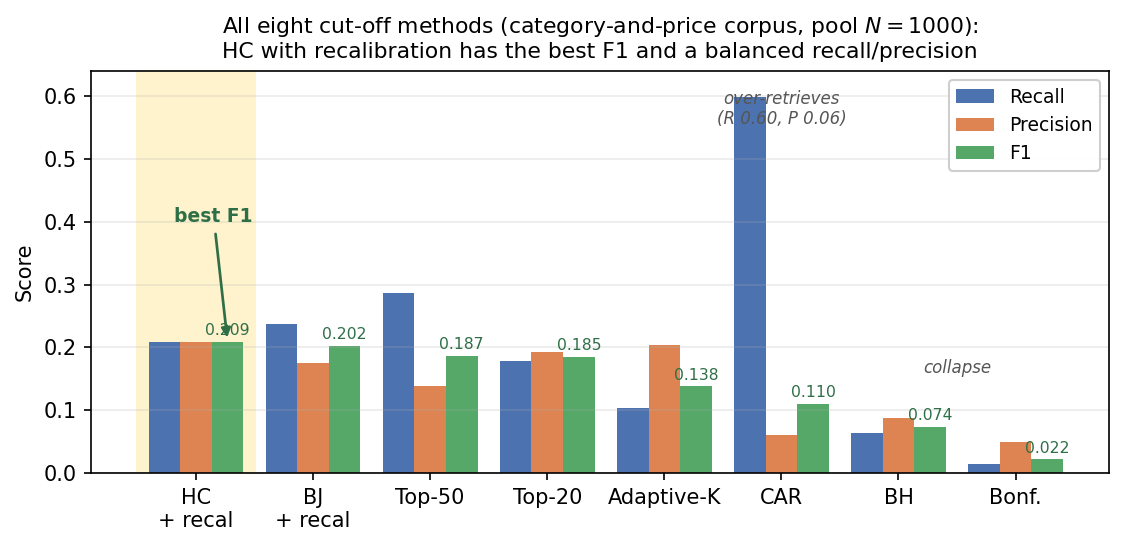
\includegraphics[width=\linewidth]{figures/fig_methodcompare.png}
\caption{All eight cut-off methods on the category-and-price corpus
(pool $N{=}1000$). HC with recalibration (highlighted) has the best F1
and a balanced recall/precision; the cluster rule (CAR) over-retrieves
to a high recall but near-zero precision, and the family-wise-error
(Bonferroni) and false-discovery (BH) rules collapse to almost nothing.}
\label{fig:methodcompare}
\end{figure}

\subsection{Best in class, and it generalizes}

\begin{table}[t]
\centering\small
\setlength{\extrarowheight}{1.5pt}
\begin{tabular}{|l|c|c|c|c|}
\hline
\textbf{Method} & \textbf{R} & \textbf{P} & \textbf{F1} & \textbf{$k$} \\
\hline
Top-20 & 0.179 & 0.192 & 0.185 & 20 \\
\hline
Top-50 & 0.287 & 0.139 & 0.187 & 50 \\
\hline
Adaptive-K (gap) & 0.104 & 0.204 & 0.138 & 9 \\
\hline
CAR (cluster) & 0.598 & 0.060 & 0.110 & 417 \\
\hline
Bonferroni & 0.014 & 0.049 & 0.022 & 0.3 \\
\hline
Benjamini--Hochberg & 0.064 & 0.087 & 0.074 & 1.6 \\
\hline
Berk--Jones + recal & 0.238 & 0.176 & 0.202 & 35 \\
\hline
\textbf{HC + recal} & 0.209 & 0.209 & \textbf{\AlgHCF} & 34 \\
\hline
\end{tabular}
\caption{Phase-2, category-and-price corpus (80K docs, pool $N{=}1000$).
HC with recalibration is the only method whose F1 beats every fixed
Top-$k$; the cluster rule over-retrieves ($k{=}417$) and the
multiple-testing rules collapse to a handful of documents.}
\label{tab:p2cp}
\end{table}

With the recalibration in place, HC is the only method whose F1 beats
every fixed Top-$k$ on the category-and-price corpus, at a moderate mean
$k{=}34$ (Table~\ref{tab:p2cp}). The
contrast with the other adaptive
rules is instructive. The clustering rule over-retrieves to hundreds of
documents and the classical multiple-testing rules under-retrieve to
almost none, so neither finds a useful operating point; only the
goodness-of-fit statistics (HC, and Berk--Jones behind it) sit where a
liberal-but-precise cutoff should. The advantage is not a small-corpus
artifact. On the 100{,}000-document electronics corpus HC again takes the
best retrieval F1 (\AmElHCF\ vs.\ \AmElTwentyF\ and \AmElFiftyF\ for fixed
Top-20/50), and the gain carries through generation: with
\texttt{gpt-5-mini} it improves answer token-F1 by $+\AmElTokF\%$ over a
fixed Top-20 and reaches 94--97\% of a much larger Top-50 cut's quality
while reading about a third fewer documents (Figure~\ref{fig:electronics}).

\begin{figure}[t]
\centering
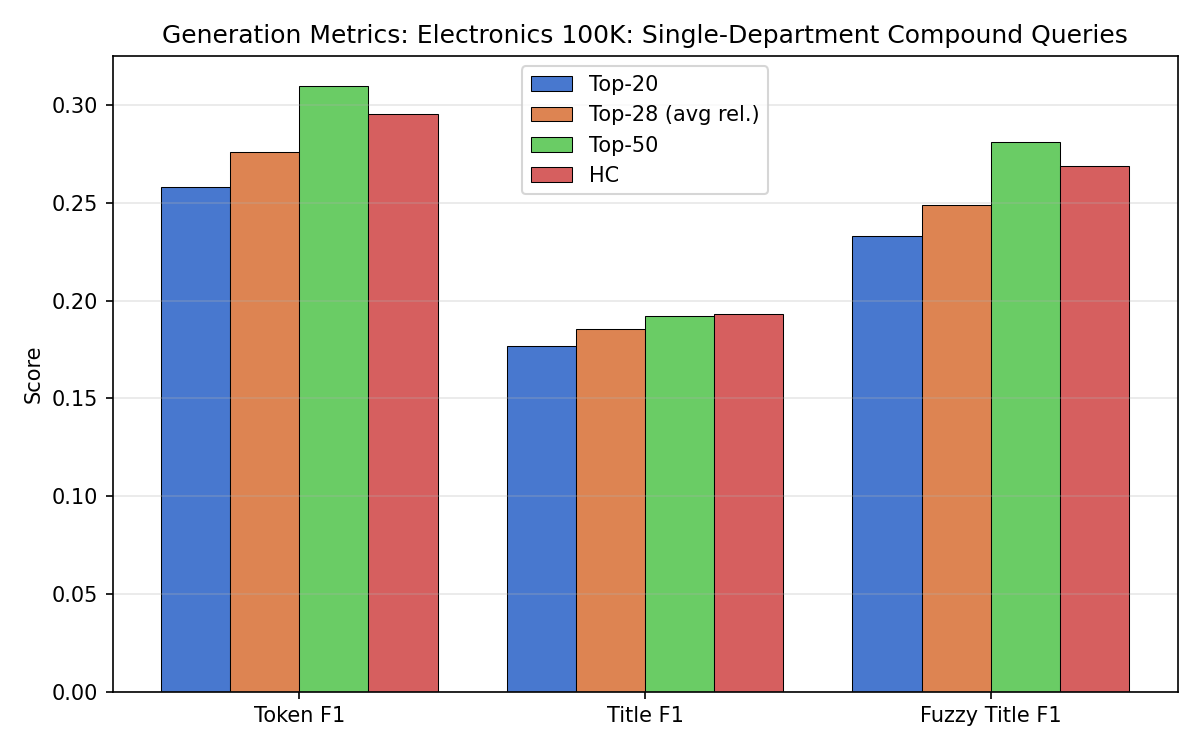
\includegraphics[width=\linewidth]{figures/fig_electronics_qa.png}
\caption{End-to-end generation on the 100K electronics corpus. HC reaches
94--97\% of a fixed Top-50 cut's answer quality while retrieving about a
third fewer documents, and improves on Top-20 across token-, title-, and
fuzzy-title-F1.}
\label{fig:electronics}
\end{figure}

\paragraph{Answering the presentation feedback.} Our final-presentation
feedback raised a specific concern: an HC cutoff should be more liberal
than a fixed one, giving higher recall and lower precision, yet our early
Amazon results showed the opposite, which the feedback attributed to a
problem in the null evaluation and asked us to check by verifying
$p$-value uniformity. The controlled study answers this. The negative-HC
collapse is the symptom of inflated $p$-values, the scale mismatch is its
measured cause, and the recalibration restores the expected recall-up,
precision-down behaviour. We also verify uniformity directly: under an
empirical null the non-relevant $p$-values are uniform, whereas a
parametric normal null is not (\ref{app:null}).

%====================================================================
% === Conclusions ===
%====================================================================
\section{Conclusions and Future Work}
Higher Criticism is a competitive query-adaptive cutoff whose behaviour
is governed by the null distribution that turns similarities into
$p$-values and fixes the threshold. That dependence is true by
construction; what matters is a precise, measured account of how the null
behaves at the boundary of detectability \cite{donohojin2004hc}. In a
controlled setting we showed how a single global null, the
production-realistic requirement that a deployable retriever calibrate
once and generalize to unseen queries, fails on hard queries through a
per-query scale mismatch, and we corrected it with a label-free
recalibration that needs no labels and keeps one global null. The
recalibrated method gives the best retrieval F1 of any we tested
($\AlgHCF$, the only one to beat every fixed Top-$k$), and the advantage
holds to 100{,}000 documents and through to generated answers.

The residual failures are embedding-limited, not statistical: when a
query turns on a numeric attribute the embedding cannot encode, no test
recovers an absent signal. The natural next step is hybrid retrieval that
pairs embeddings for category semantics with structured metadata
filtering for the numeric constraint, with a per-query null for small
clustered corpora and a benchmark-wide $p$-value uniformity diagnostic as
further directions. A week-by-week roadmap is in \ref{app:roadmap}.

%====================================================================
% === References ===
%====================================================================
\bibliographystyle{plain}
\bibliography{refs}

%====================================================================
% === Appendices ===
%====================================================================
\appendix
\renewcommand{\thesection}{Appendix~\Alph{section}}

\section{Project Roadmap}
\label{app:roadmap}
\small
\begin{tabular}{@{}p{0.05\linewidth}p{0.88\linewidth}@{}}
\toprule
\textbf{Wk} & \textbf{Milestone / Outcome} \\
\midrule
4   & \textbf{Foundations.} Implemented the HC module ($p$-values from a per-query null, $\gamma$ guardrail) and the indexing stack on the CRAG \cite{crag2024} corpus (recursive chunking, 384/50 overlap; OpenRouter LLM interface). \emph{Direction change:} a $k$-sweep with \texttt{all-mpnet-base-v2} favoured $k{=}10$, but BGE \cite{bgeembeddings2023} gave a clear recall lift on a 1K-doc subset, so BGE became the default embedder. \\
5   & \textbf{Survey of adaptive retrievers.} Catalogued competing approaches (Reciprocal Rank Fusion, CAR \cite{xu2025car}, uncertainty filtering) to position HC as a global, distribution-aware test, and fixed the comparison set (Bonferroni \cite{bonferroni1961dunn}, Benjamini--Hochberg \cite{benjamini1995fdr}, gap-based Adaptive-K \cite{adaptivek2025}). First HC vs.\ Top-K runs. \\
6   & \textbf{Long-context regime: HoloBench.} First HC vs.\ gap-based Adaptive-K on HoloBench \cite{maekawa2024holobench}. Judge scores tracked closely; \emph{iteration:} diagnosed as a generation/judge bottleneck on aggregation, not a retrieval tie, which motivated stronger retrieval-only metrics. \\
7   & \textbf{Multi-hop regime + dataset-aware $\gamma$.} Repeated on HotpotQA \cite{yang2018hotpotqa}. \emph{Change in direction:} a stark dense-vs-sparse asymmetry meant the same $\gamma$ behaved very differently, so $\gamma$ was treated as dataset-aware. Began Adaptive-RAG \cite{jeong2024adaptiverag} and FlashRAG \cite{jin2025flashrag} integration. \\
8   & \textbf{Pipeline integrations + FiQA.} Plugged HC into Adaptive-RAG as a fourth strategy; on HotpotQA it beat single-step \textsc{oneR} and lost to multi-step \textsc{ircot}, as expected. Registered HC and Berk--Jones \cite{berkjones1979} as FlashRAG post-processors on BEIR SciFact \cite{thakur2021beir,wadden2020scifact}, FiQA \cite{thakur2021beir}, and MS MARCO. \emph{Iteration:} FiQA was the first single-hop negative result and triggered the position study behind the scattered-relevance analysis. \\
9   & \textbf{CrossEntityQA construction.} \emph{Change in direction:} rather than keep tuning on off-the-shelf data, we built a sparse-relevance benchmark to surface HC's target regime (SPARQL Wikidata clusters $\to$ Wikipedia passages $\to$ LLM queries answerable only by aggregating several passages; $\sim$2\% relevance, controllable $K$). \\
10  & \textbf{Negative result: CrossEntityQA + BM25.} HC \emph{lost} to fixed Top-5 under BM25, whose score magnitude encodes lexical match, not the categorical constraints these queries impose. \emph{Change in direction:} dropped BM25 for CrossEntityQA and committed to a dense retriever. \\
11  & \textbf{Final breadth head-to-head.} With the dense pipeline HC won on passage F1 on CrossEntityQA (Table~\ref{tab:p1a}) and was competitive with single-step retrieval on MuSiQue \cite{trivedi2022musique}, closing the breadth picture and motivating the controlled Amazon study. \\
\bottomrule
\end{tabular}
\normalsize

\section{HC-RAG Pipeline}
\label{app:pipeline}
Figure~\ref{fig:pipeline} shows the full offline/online pipeline; every
pipeline in this report differs only in the HC-cutoff box.

\begin{figure}[h]
\centering
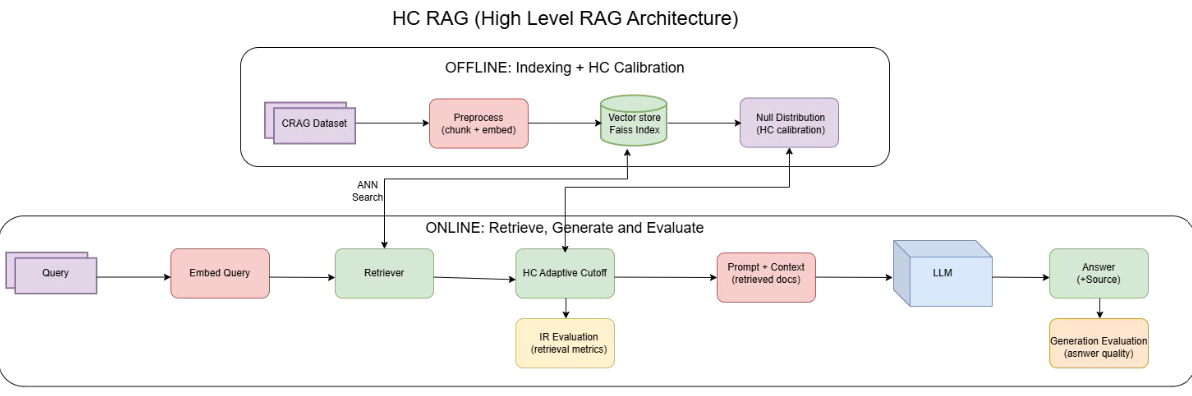
\includegraphics[width=\linewidth]{figures/rag_pipeline.png}
\caption{The HC-RAG pipeline. \emph{Offline:} chunk and embed the corpus,
build a FAISS \cite{johnson2019faiss} index, and calibrate the null.
\emph{Online:} embed the query, retrieve a candidate pool, apply the HC
cutoff, and pass the selected passages to the LLM; retrieval and
generation are both evaluated.}
\label{fig:pipeline}
\end{figure}

\section{Comparison Methods}
\label{app:methods}
Table~\ref{tab:methods} lists the selection rules compared in the study.
``Concept'' is the rule that turns a candidate pool into a document set;
the statistical methods share HC's $p$-value machinery and differ only in
the decision rule.

\begin{table}[h]
\centering\small
\begin{tabular}{@{}lll@{}}
\toprule
\textbf{Method} & \textbf{Concept} & \textbf{Reference} \\
\midrule
Fixed Top-$k$        & rank cutoff                & --- \\
Adaptive-K           & largest score gap          & \cite{adaptivek2025} \\
Adaptive-RAG         & complexity routing         & \cite{jeong2024adaptiverag} \\
FlashRAG post-proc.  & cutoff plug-in             & \cite{jin2025flashrag} \\
Full-context         & all chunks to the LLM      & --- \\
Self-route           & retrieve + routing prompt  & --- \\
\textbf{HC} (ours)   & Higher Criticism statistic & \cite{donohojin2004hc} \\
Berk--Jones          & goodness-of-fit statistic  & \cite{berkjones1979} \\
Bonferroni           & FWER threshold             & \cite{bonferroni1961dunn} \\
Benjamini--Hochberg  & FDR step-up                & \cite{benjamini1995fdr} \\
CAR                  & cluster cutoff             & \cite{xu2025car} \\
\textbf{Per-query recal.} (ours) & rescale $z$-scores to the global null & --- \\
\bottomrule
\end{tabular}
\caption{Methods compared. All share HC's $p$-value machinery except the
fixed and cluster rules.}
\label{tab:methods}
\end{table}

\section{CrossEntityQA Construction}
\label{app:ceqa}
Figure~\ref{fig:ceqa} shows the CrossEntityQA construction pipeline. It
guarantees a controllable per-query relevance count ($K{=}2$--20) and a
sparse corpus (about 2\% relevant), the two properties that make the
benchmark a stress test for adaptive-$k$ retrieval. Generation code is in
\texttt{dataset\_builders/cross\_entity\_qa/}.

\begin{figure}[h]
\centering
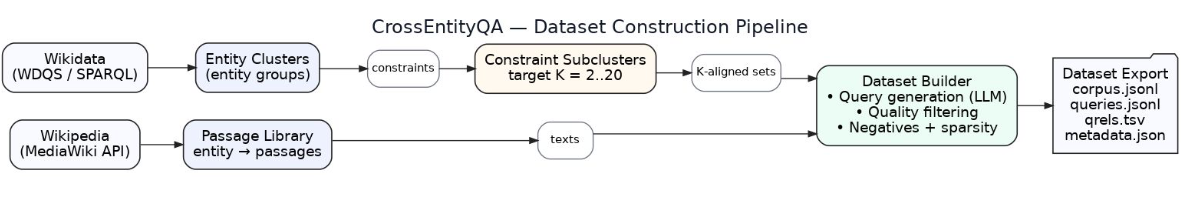
\includegraphics[width=\linewidth]{figures/cross_entity_qa.png}
\caption{CrossEntityQA construction. Wikidata entity groups (WDQS/SPARQL)
are split into constraint subclusters with a target relevance count
$K{=}2$--20; a Wikipedia passage library supplies the texts; the builder
generates LLM queries, filters for quality, and controls negatives and
sparsity, exporting corpus, queries, and qrels.}
\label{fig:ceqa}
\end{figure}

\section{Null-Distribution Diagnostics}
\label{app:null}
This appendix answers the presentation feedback to verify that the
$p$-values are uniform under the null. On BEIR FiQA, under the
\emph{empirical} null the non-relevant $p$-values are uniform
(KS $p{=}0.13$; 5.0\% below 0.05), whereas a \emph{parametric normal}
null is not (KS $p{=}0.000$, an excess spike near zero), which is why we
keep the empirical null; relevant documents carry systematically small
$p$-values (Cohen's $d{=}{-}1.33$), and the QQ plot of empirical
$p$-values sits on the uniform diagonal (Figure~\ref{fig:nulldiag}).

\begin{figure}[h]
\centering
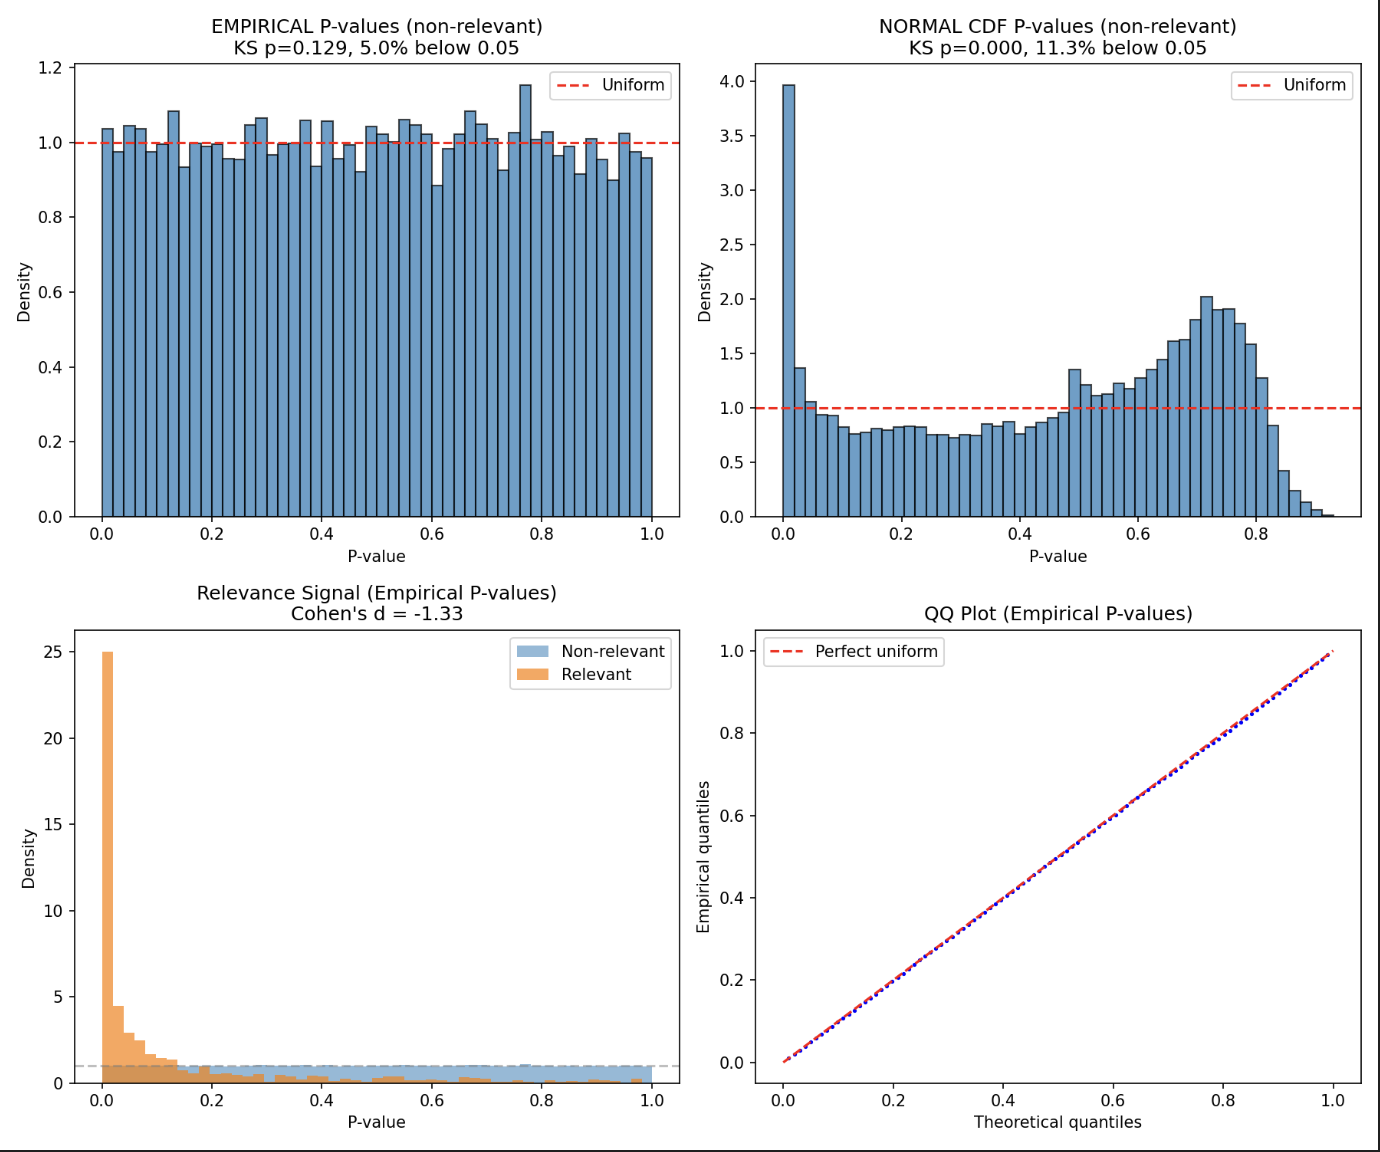
\includegraphics[width=\linewidth]{figures/fiqa_null_pvalues.png}
\caption{$p$-value uniformity diagnostics under the null (BEIR FiQA). The
empirical null is uniform (top-left; QQ bottom-right) while a parametric
normal null is not (top-right); relevant documents separate in $p$-value
space (bottom-left). This is the uniformity check requested in the
presentation feedback.}
\label{fig:nulldiag}
\end{figure}

\end{document}
